\documentclass[a4paper,12pt]{report}

\usepackage[utf8x]{inputenc}
\usepackage[T2A]{fontenc}
\usepackage[english, russian]{babel}
\usepackage[table]{xcolor}

% Опционно, требует  apt-get install scalable-cyrfonts.*
% и удаления одной строчки в cyrtimes.sty
% Сточку не удалять!
% \usepackage{cyrtimes}

% Картнки и tikz
\usepackage{graphicx}
\usepackage{tikz}
\usetikzlibrary{snakes,arrows,shapes}


% Увы, поля придётся уменьшить из-за листингов.
\topmargin -1cm
\oddsidemargin -0.5cm
\evensidemargin -0.5cm
\textwidth 17cm
\textheight 24cm

\sloppy



% Оглавление в PDF
\usepackage[
bookmarks=true,
colorlinks=true, linkcolor=black, anchorcolor=black, citecolor=black, menucolor=black,filecolor=black, urlcolor=black,
unicode=true
]{hyperref}

% Для исходного кода в тексте
% \newcommand{\Code}[1]{\texttt{#1}}

% Некоторая русификация.
% \usepackage{misccorr} % Oh shi^W^W, оно не работает с report.
\usepackage{indentfirst}
\renewcommand{\labelitemi}{\normalfont\bfseries{--}}

% На дворе XXI век, но пакет listings всё ещё не пашет с русскими комментариями!

% Пакет listings для простой вставки исходников
% \usepackage{listings}
% Параметры оформления
% \lstset{
% showspaces=false,
% showtabs=false,
% frame=single,
% tabsize=4,
% basicstyle=\ttfamily,
% identifierstyle=\ttfamily,
% commentstyle=\itshape,
% stringstyle=\ttfamily,
% keywordstyle=\ttfamily,
% breaklines=true
% }
% Русский в комментариях.
% \lstset{escapebegin=\begin{cyr},escapeend=\end{cyr}}



% А это взято из файла, сгенерённого doxygen
% Packages required by doxygen
\usepackage{fixltx2e}
\usepackage{calc}
\usepackage{doxygen}
\usepackage{graphicx}
\usepackage{makeidx}
\usepackage{multicol}
\usepackage{multirow}
\PassOptionsToPackage{warn}{textcomp}
\usepackage{textcomp}
\usepackage[nointegrals]{wasysym}
\usepackage{ifpdf,ifxetex}

% NLS support packages
\usepackage[T2A]{fontenc}
\usepackage[russian]{babel}

% Font selection
\usepackage[T1]{fontenc}
\usepackage[scaled=.90]{helvet}
\usepackage{courier}
\usepackage{amssymb}
\usepackage{sectsty}
\renewcommand{\familydefault}{\sfdefault}
\allsectionsfont{%
  \fontseries{bc}\selectfont%
  \color{darkgray}%
}
\renewcommand{\DoxyLabelFont}{%
  \fontseries{bc}\selectfont%
  \color{darkgray}%
}
\newcommand{\+}{\discretionary{\mbox{\scriptsize$\hookleftarrow$}}{}{}}

% Arguments of doxygenemoji:
% 1) ':<text>:' form of the emoji, already "LaTeX"-escaped
% 2) file with the name of the emoji without the .png extension
% in case image exist use this otherwise use the ':<text>:' form
\newcommand{\doxygenemoji}[2]{%
  \IfFileExists{./#2.png}{\raisebox{-0.1em}{\includegraphics[height=0.9em]{./#2.png}}}{#1}%
}
% Page & text layout
\usepackage{geometry}
\geometry{%
  a4paper,%
  top=2.5cm,%
  bottom=2.5cm,%
  left=2.5cm,%
  right=2.5cm%
}
\tolerance=750
\hfuzz=15pt
\hbadness=750
\setlength{\emergencystretch}{15pt}
\setlength{\parindent}{0cm}
\newcommand{\doxynormalparskip}{\setlength{\parskip}{3ex plus 2ex minus 2ex}}
\newcommand{\doxytocparskip}{\setlength{\parskip}{1ex plus 0ex minus 0ex}}
\doxynormalparskip
\makeatletter
\renewcommand{\paragraph}{%
  \@startsection{paragraph}{4}{0ex}{-1.0ex}{1.0ex}{%
    \normalfont\normalsize\bfseries\SS@parafont%
  }%
}
\renewcommand{\subparagraph}{%
  \@startsection{subparagraph}{5}{0ex}{-1.0ex}{1.0ex}{%
    \normalfont\normalsize\bfseries\SS@subparafont%
  }%
}
\makeatother

% Indices & bibliography
\usepackage{natbib}
\usepackage[titles]{tocloft}
\setcounter{tocdepth}{3}
\setcounter{secnumdepth}{5}
\makeindex

\usepackage{newunicodechar}
  \newunicodechar{⁻}{${}^{-}$}% Superscript minus
  \newunicodechar{²}{${}^{2}$}% Superscript two
  \newunicodechar{³}{${}^{3}$}% Superscript three

% Custom commands
\newcommand{\clearemptydoublepage}{%
  \newpage{\pagestyle{empty}\cleardoublepage}%
}

\usepackage{caption}
\captionsetup{labelsep=space,justification=centering,font={bf},singlelinecheck=off,skip=4pt,position=top}

\usepackage{etoc}
\etocsettocstyle{\doxytocparskip}{\doxynormalparskip}
\renewcommand{\numberline}[1]{#1~}


\title{Отчёт по курсовой работе}
\author{Горин Дмитрий Игоревич}

\begin{document}

\maketitle

\tableofcontents

\addcontentsline{toc}{chapter}{Введение}
\chapter*{Введение}

Задание на курсовую работу: Реализовать клиента SMTP-сервера с использованием системного вызова \textit{select} и использующего один рабочий поток с журналированием в отдельном процессе.
Данный отчет содержит информацию о протоколе \textit{SMTP}, а так же информацию о реализации и разработке курсового проекта.

\chapter{Аналитический раздел}

\section{Протокол SMTP}

SMTP (Simple Mail Transfer Protocol) — это широко используемый сетевой протокол, предназначенный для передачи электронной почты в сетях TCP/IP.
SMTP впервые был описан в RFC 821 (1982 год); последнее обновление в RFC 5321 (2008) включает масштабируемое расширение — ESMTP (Extended SMTP).
В настоящее время под «протоколом SMTP» как правило подразумевают и его расширения.
Протокол SMTP предназначен для передачи исходящей почты с использованием порта TCP 25.

\subsection{SMTP-команды}

Ниже представлен неплоный список SMTP-команд:
\begin{itemize}
    \item \textit{HELO} - Открывает SMTP-сессию
    \item \textit{EHLO} - Открывает ESMTP-сессию
    \item \textit{MAIL} - Определяет отправителя сообщения
    \item \textit{RCPT} - Определяет получателей сообщения
    \item \textit{DATA} - Определяет начало сообщения
    \item \textit{RSET} - Сброс SMTP-соединения
    \item \textit{VRFY} - Проверяет имя пользователя системы
    \item \textit{QUIT} - Остановить сеанс SMTP
\end{itemize}

\subsection{SMTP-сессия}
SMTP-сессия состоит из команд, посылаемых SMTP-клиентом, и соответствующих ответов SMTP-сервера.
Когда сессия открыта, сервер и клиент обмениваются её параметрами.
Сессия может включать ноль и более SMTP-операций (транзакций).

Сессия начинается с команды \textit{HELO} или \textit{EHLO}, и заканчивается командой \textit{QUIT}.
Сбросить состояние сессии можно командой \textit{RSET}.

Отправка сообщения состоит из трёх последовательностей команда/ответ:
\begin{enumerate}
    \item \textit{MAIL FROM} — устанавливает обратный адрес
    \item \textit{RCPT TO} — устанавливает получателя данного сообщения.
    Эта команда может быть дана несколько раз, по одной на каждого получателя.
    \item \textit{DATA} — для отправки текста сообщения.
\end{enumerate}

\section{Плюсы и минусы использования однопоточной схемы обработки подключений с использованием системного вызова select}
Плюсы:
\begin{itemize}
    \item Упрощение логики программы
    \item select принимает аргументы одной длинны, что упрощает работу с памятью
\end{itemize}

Минусы:
\begin{itemize}
    \item select может обработать до 1024 (FD\_SETSIZE) подключений максимум
    \item Невозможна одновременная (параллельная) обработка нескольких подключений, что увеличит время обработки каждого подключения
\end{itemize}

\chapter{Конструкторский раздел}

\section{Конечный автомат состояний сервера}

На Рис.~\ref{fig:fsm-client} представлен конечный автомат клиентской части курсовой работы.

\begin{figure}
    \centering
    \includegraphics[width=\textwidth]{include/fsm.pdf}
    \caption{Состояния клинетской части}
    \label{fig:fsm-client}
\end{figure}

\section{Описание основных структур данных}
\begin{itemize}
    \item String -- Структура строки текста
    \item SMTPMessage -- SMTP-сообщение. Содержит весь текст сообщения, а так же спарсенные данные для команд MAIL FROM и RCPT TO
    \item SMTPMessageQueue -- Очередь SMTP-сообщений
    \item SMTPConnection -- SMTP-соединение. Содержит сокет, буферы чтения и записи и очередь сообщений
    \item SMTPConnectionList -- Список SMTP-подключений
\end{itemize}

\begin{figure}
    \centering
    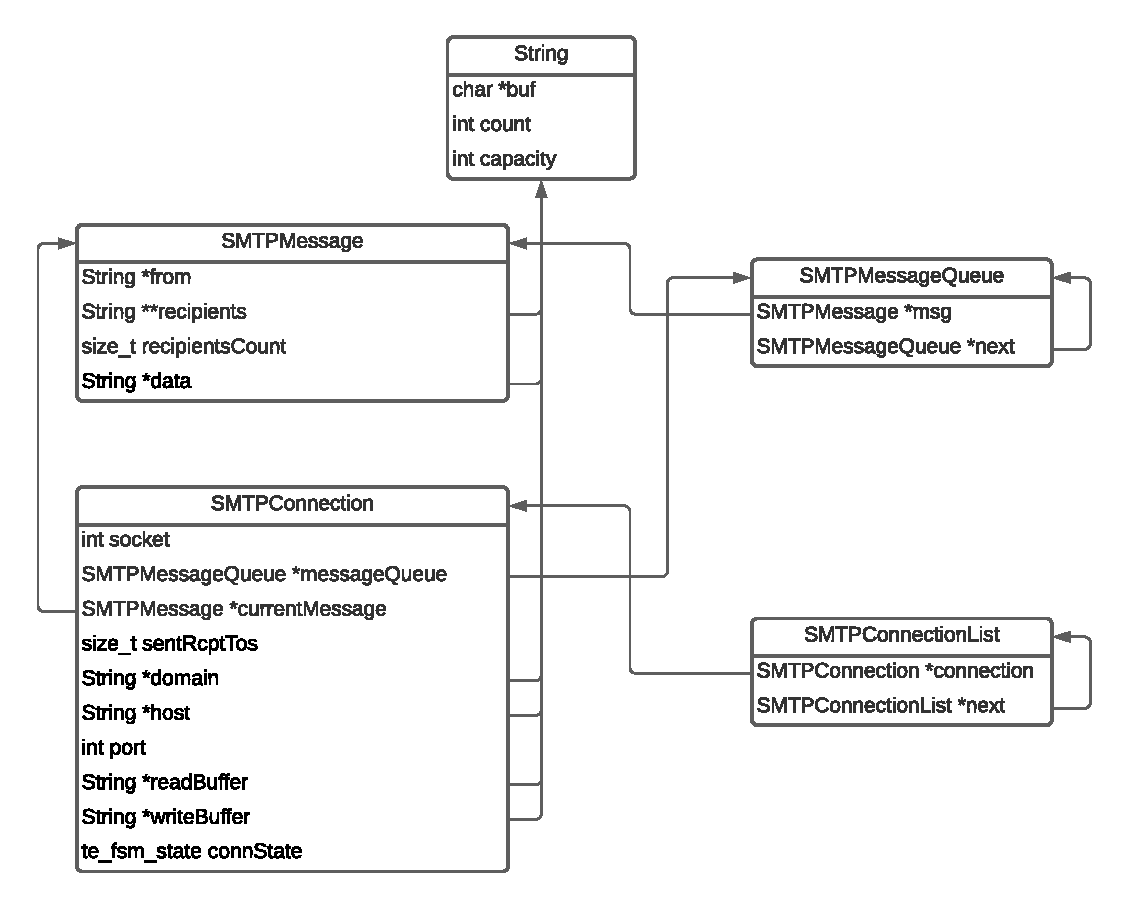
\includegraphics[width=\textwidth]{include-git/SMTP-ER.pdf}
    \caption{ER-диаграмма}
    \label{fig:er}
\end{figure}

\section{Связь логгера и основной программы}
Программа-клиент отправляет сообщения программе-логгеру через технологию IPC message queue (sys/msg.h)


%\section{Синтаксис команд протокола}

%\begin{description}
%\item[Команда выхода из сеанса]
%%\input{include/re_cmd_quit_re.tex}
%Вот тут было вот такое \(\\input\{include/re_cmd_quit_re.tex\}\), но закоментил
%\item[Команда передачи имени пользователя]
%Тут тоже примерно такое
%%\input{include/re_cmd_user_re.tex}
%\end{description}
%
%Для грамматики можно использовать вставку из файла и оформление \textbackslash{}begin\{verbatim\} и \textbackslash{}end\{verbatim\} или пакет \textit{listings}\footnote{На дворе XXI век, но пакет \textit{listings} всё ещё не пашет с русскими комментариями без бубна, и лично я его пока не победил.}.
%
%Для примера воспользуемся автоматической вставкой файла описания параметров программы \(не забудьте перенести это в технологический раздел\) через утилитку \textit{src2tex}.
%
%Ну у меня аутоопс нет, так что закомментил это: \(\\input\{include/checkoptn.def.tex\}\)
%% \lstset{language=C}
%% \lstinputlisting{../src/checkoptn.def}

\chapter{Технологический раздел}

\section{Доступ к данным на диске}
Сервер записывает все письма в директорию Client/mails в виде текстовых файлов.
Для корректной работы команд MAIL FROM и RCPT TO сервер записывает нужные данные в заголовки X-KIMI-From и X-KIMI-To соответственно.

\section{Сборка программы}
Сборка программы описана в файле \textit{Makefile} системы сборки \textit{make}.
%Рис.~\ref{fig:make} нагенерили самодельные \textit{makesimple} и \textit{makefile2dot}, а также \textit{dot2tex} и \textit{dot}.

%\begin{figure}
%\centering
%\includegraphics[width=\textwidth]{include/makefile.pdf}
%\caption{Сборка программы}
%\label{fig:make}
%\end{figure}

%Отмечу, что за исключения целей типа \textit{all}, \textit{install}, \textit{clean}, \textit{tests}, все имена целей в файле систем сборки \textit{make} обычно совпадают с именами файлов \(такой вот низкоуровневый инструмент\). То есть вместо цели \textit{lexer} следует использовать цель \textit{src/lexer.c}.

\section{Основные функции программы}

Весь это раздел сгеренерировал doxygen из части комментированных исходников программы.
В файле конфигурации \textbf{doxyggen.cfg} был отключён параметр \textbf{HAVE\_DOT}, поскольку для рисования графов вызовов используется \textit{cflow}.

\input{include/doxygen/latex/client_8c.tex}
\input{include/doxygen/latex/logger_8c.tex}
\input{include/doxygen/latex/smtp__connection_8c.tex}
\input{include/doxygen/latex/smtp__connection__list_8c.tex}
\input{include/doxygen/latex/smtp__message_8c.tex}
\input{include/doxygen/latex/smtp__message__queue_8c.tex}


\section{Графы вызова функций}

На рис.~\ref{fig:cflow01} показаны основные функции.
%Файл \textbf{cflow.ignore} содержит список функций \(точнее, шабловнов поиска\), использыемых программой \textit{grep} для удаления малоинтересных стандартных функций\footnote{Функции по работе с сокетами, ipc и привилегиями к малоинтересным ни в коем случае не относятся.}.

\begin{figure}[H]
    \centering
    \includegraphics[width=\textwidth]{include/cflow.pdf}
    \caption{Граф вызовов, основные функции клиента}
    \label{fig:cflow01}
\end{figure}

Графы созданы с помощью \textit{cflow}, \textit{cflow2dot}, \textit{dot}.

\section{Модульные тесты}
Для модульного тестирования используется библиотека CUnit. Всего написано 35 тестов с 205 ASSERT-вызовами.

\section{Проверка утечек памяти с помощью valgrind}
    \begin{verbatim}
        ==33081== HEAP SUMMARY:
        ==33081== in use at exit: 962,565 bytes in 14,919 blocks
        ==33081== total heap usage: 18,623 allocs, 3,704 frees, 1,026,349 bytes allocated
        ==33081==
        ==33081== Searching for pointers to 14,919 not-freed blocks
        ==33081== Checked 14,649,888 bytes
        ==33081==
        ==33081== LEAK SUMMARY:
        ==33081== definitely lost: 0 bytes in 0 blocks
        ==33081== indirectly lost: 0 bytes in 0 blocks
        ==33081== possibly lost: 0 bytes in 0 blocks
        ==33081== still reachable: 944,640 bytes in 14,760 blocks
        ==33081== suppressed: 17,925 bytes in 159 blocks
        ==33081== Rerun with —leak-check=full to see details of leaked memory
        ==33081==
        ==33081== ERROR SUMMARY: 0 errors from 0 contexts (suppressed: 4 from 4)
    \end{verbatim}

\section{Генерация документации и отчета}
Отчет и документация генерируются автоматически через Makefile.
Для этого в Makefile добавлена цель doxygen и report (report также генерирует doxygen).

\addcontentsline{toc}{chapter}{Выводы}
\chapter*{Выводы}

В ходе выполнения работы был реализован клиент серверной части SMTP-сервера.
Был изучен протокол SMTP и были получены навыки в написании сетевых приложений на языке C с использованием мультиплексирования.

\end{document}
